\section{Исследование и построение решений задачи}
\label{sec:Chapter_4} \index{Chapter_4}
\large




\subsection{Шаблонный метод}

Для тестирования первого метода решения поставленной задачи, необходимо
было составить шаблоны поиска гипонимов и гиперонимов, аналогичных шаблонам
Марти Херст.

Были найдены уже готовые примеры шаблонов как в научных статьях, так и в
готовых программах, написанных на языке программирования. Наиболее широки
списком разнообразных шаблонов обладал класс \textit{hearstPatterns}, написанный на
языке Python. Всего в нем содержалось 48 примеров, написанных регулярными
выражениями.

Для удобной и более быстрой работы с данным классом, необходимо было
выгрузить исходный код и подправить его под свою задачу. Производилась
внутренняя лемматизация слов и приведение их к нижнему регистру, а также
удаление пунктуации предложения. В итоге, была получена функция, на вход
которой передавалось необработанное предложение, а на выходе составлялся
список найденных пар гипоним-гипероним.
Целью проверки данного метода шаблонов было извлечение всех пар, связанных
отношением is-a, из текстового корпуса UMBC средствами класса \textit{hearstPattern}s, и
последующая оценка выбранными метриками.

Как оказалось на практике, написанных шаблонов было недостаточно, для
качественного обнаружения искомых пар. В качестве примера: из 1,5 млн
предложений было обнаружено всего 8003 пары. Более того, на обработку одно
предложения всеми регулярными выражениями требовалось очень много времени.
Просмотр всего корпуса требовал более 5-ти дней. Поэтому добавление новых
рукописных шаблонов не представлялось возможным.

Результаты:

\begin{itemize}
\item MRR: 0.005
\item MAP: 0.0017
\item P@1: 0.0033
\item P@3: 0.0023
\item P@5: 0.0018
\item P@15: 0.0012
\end{itemize}

Не имея в наличии мощной техники, достаточного времени и богатого списка
шаблонов, протестировать данной метод в полном объеме не удалось.





\subsection{PPMI + SVD}

Для исследования первого метода, основанного на дистрибутивной гипотезе, каждое
предложение текстового корпуса было разбито на контексты с шириной окна в 5 слов.
Составлена разреженная матрица частоты встречаемости пары (слово, контекст). Затем
полученная матрица была пересчитана в PPMI матрицу по формулам, описанным в пункте
2.1.

Размер матрицы оказался слишком большим, чтобы было возможно применить алгоритм
снижения размерности SVD. Были опробованы готовые реализации модели на языках
Python (классы numpy.linalg.svd и scipy.sparse.linalg.svds) и Matlab (svd), но ни одна из них не смогла преобразовать PPMI матрицу.

Таким образом, метод PPMI + SVD, получения векторного представления слов,
протестировать на существующий данных не удалось.





\subsection{WORD2VEC}

\subsubsection{Модель GOOGLENEWS}

Следующим исследуемым методом получения векторного представления слов был
Word2Vec.
Существует множество готовых обученных моделей, опубликованных в открытом доступе.
Для тестирования решения данной задачи была применена модель, имеющая архитектуру
CBOW и обученная на корпусе GoogleNews, размером в 3 миллиона слов. Основные
параметры: размерность вектора 300, размер окна 5.
Алгоритм Word2Vec основывается на информации о контекстах, в которых употреблялось
слово в текстовом корпусе, поэтому получение вектора возможно только для тех слов,
которые встречались в корпусе хотя бы 1 раз (в общем случае, не менее N раз, где порог N
является гиперпараметром). Значит, если гипоним, для которого необходимо найти все
гиперонимы, не встречался, в обучающем корпусе, то построенная модель не сможет
подобрать для него требуемый список.
Из 1500 гипонимов, находящихся в выбранном корпусе данных, построенная модель,
смогла предоставить вектора только для 77%. Для оставшихся слов, необходимо было
применять другую модель.
Для получиния итогового списка гиперонимов к каждому гипониму, было применено 2
различных алгоритма: GBR (Gradient Boosting for regression) и LambdaRank.
Алгоритм GBR можно применить как pointwise алгоритм ранжирования. В то время как
LambdaRank является представителем pairwise подхода. Нельзя заранее сказать, какой из
двух подходов будет работать лучше, поэтому для тестирования были использованы оба.

\paragraph{Подготовка обучающего множества}
~\
~\

Так как необходимо было исследовать множество алгоритмов с различными параметрами,
для экономии скорости и минимальной потери точности, извлечение гиперонимов
происходило не из полного словаря, содержащего $\approx 220$ тыс слов. Для каждого гипонима
составлялся свой словарь по следующему алгоритму:

\begin{enumerate}
\item Добавлялись все слова из эталонного списка гиперонимов. Среднее количество
гиперонимов для каждого гипонима составляло 5 слов

\item Каждому слову из списка присваивалось значение, отражающее его позицию. Эти
величины служат целевым признаком для предсказания. Для алгоритма
LambdaRank чаще всего используются значения 0,1,2 и 3, поэтому для эталонных
гиперонимов были выбраны значения 1,2 и 3. Список делился на три части, если
слово находилось в первой из них, то ему присваивалась величина 3, если во
второй, то 2, оставшейся последней части - 1.

\item Далее в случайном порядке добавлялось к полученному списку дополнительно 500
слов, играющих роль негативных примеров. Каждое такое слово имело целевое
значение 0.
\end{enumerate}

В качестве признаков для обучения моделей были протестированны следующие
комбинации векторов гипонима и гиперонима:

\begin{enumerate}
\item Разность векторов
$Diff: <u - v>$

\item Конкатенация векторов + евклидово расстояние степени 1
$||u - v||_1 = \sum_{i=1}^{|u_i - v_i|}$
$Dist1: <u, v, ||u - v||_1>$

\item Конкатенация векторов + евклидово расстояние степени 2
$||u - v||_2 = \sqrt{\sum_{i=1}^{|(ui - vi)^2|}}$
$Dist2: <u, v, || u - v ||_2>$

\item Конкатенация векторов + косинусное расстояние между ними
$Cos: <u, v, cos(u, v)>$
\end{enumerate}

Полученный новый набор данных разделялся на обучающую и тестовую выборку в
отношении 2 : 1. Так как не для всех гипонимов построены вектора, то тестирование и
обучение происходило только на 77\% данных.

\paragraph{Тестирование}
~\
~\

Получены следующие результаты:


\begin{table}[!htb]

\begin{minipage}{.5\textwidth}
\centering
%--------------------------------------
\begin{tabular}{|l|l|l|}
\hline
 & \textbf{MRR} & \textbf{MAP} \\

\hline
\textbf{Diff} & $0.914$ & $0.504$\\

\hline
\textbf{Dist1} & $0.942$ & $0.487$\\

\hline
\textbf{Dist2} & $0.914$ & $0.787$\\

\hline
\textbf{Cos} & $0.039$ & $0.044$\\

\hline
\end{tabular}
%--------------------------------------
\caption{LambdaRank}
\label{tabular:LambdaRank}
\end{minipage}%
\begin{minipage}{.5\textwidth}
\centering
%--------------------------------------
\begin{tabular}{|l|l|l|}
\hline
 & \textbf{MRR} & \textbf{MAP} \\

\hline
\textbf{Diff} & $0.893$ & $0.442$\\

\hline
\textbf{Dist1} & $0.912$ & $0.463$\\

\hline
\textbf{Dist2} & $0.918$ & $0.659$\\

\hline
\textbf{Cos} & $0.078$ & $0.062$\\

\hline
\end{tabular}
%--------------------------------------
\caption{GBR}
\label{tabular:GBR}
\end{minipage}

\end{table}


Лучший результат среди всех опробованных моделей с векторами Word2Vec - GoogleNews,
показал алгоритм LambdaRank с основными параметрами: шаг обучения = 0.1, кол-во
деревьев 100, доля выборки на каждом шаге обучения (subsample) = 0.8, максимальная
глубина 5. Для метрики MRR, более успешными было представление векторов
комбинацией Dist1, а для MAP - Dist2.

\subsubsection{Обучение собственное модели WORD2VEC}

Далее, был обучен алгоритм Word2Vec на текстовом корпусе UBMC. Целью такого
исследования было увеличение доли гипонимов, для которых возможно построить вектор,
и возможность настроить главные гиперпараметры.
Из опробованных комбинаций параметров, лучший результат показала модель Skip-gramm,
с ширеной окна 7 и размером вектора 300.
Так как среди гипонимов встречались не только слова, но и словочетания из 2-3 слов, не
удалость построить вектора для них в сех. Доля с 77\% увеличилась до 82\%.

\paragraph{Тестирование}
~\
~\

Были применены все те подходы которые использовались для эксперимента с моделью
Word2Vec - GoogleNews.
Лучшей также оказалась модель LambdaRank с теми же параметрами.
Получены следующие результаты:

\begin{table}[!htb]

\begin{minipage}{.5\textwidth}
\centering
%--------------------------------------
\begin{tabular}{|l|l|l|}
\hline
 & \textbf{MRR} & \textbf{MAP} \\

\hline
\textbf{Diff} & $0.945$ & $0.489$\\

\hline
\textbf{Dist1} & $0.931$ & $0.705$\\

\hline
\textbf{Dist2} & $0.924$ & $0.793$\\

\hline
\textbf{Cos} & $0.035$ & $0.020$\\

\hline
\end{tabular}
%--------------------------------------
\caption{LambdaRank}
\label{tabular:LambdaRank2}
\end{minipage}%
\begin{minipage}{.5\textwidth}
\centering
%--------------------------------------
\begin{tabular}{|l|l|l|}
\hline
 & \textbf{MRR} & \textbf{MAP} \\

\hline
\textbf{Diff} & $0.914$ & $0.459$\\

\hline
\textbf{Dist1} & $0.921$ & $0.588$\\

\hline
\textbf{Dist2} & $0.927$ & $0.655$\\

\hline
\textbf{Cos} & $0.081$ & $0.073$\\

\hline
\end{tabular}
%--------------------------------------
\caption{GBR}
\label{tabular:GBR2}
\end{minipage}

\end{table}



\subsection{DYNAMIC DISTANCE-MARGIN MODEL}

Для применения данного алгоритма, необходимо иметь набор триплетов $(u, v, q)$, где $u$ - гипоним, $v$ - гипероним, а $q$ - сколько раз пара гипоним-гипероним $(u, v)$ встретилась в текстовом корпусе. В качестве такого набора данных был взят ProBase, описанный в главе
шаблонных методов.

ProBase был получен на основе очень больших наборов текстовых корпусов, поэтому
значения q могли достигать величины в 35000. Алгоритм DDM (Dynamic distance-margin),
учитвает и обучает каждую пару столько раз, сколько она встречалась. Таким образом,
некоторые пары могли учитываться 35 тысяч раз за одну эпоху, в то время, как
большинство других имели значение $q < 20$. В таком случае модель могла практически не
обучить большинсво векторов. Чтобы устранить такой большой разрыв значение q было
изменено по формуле $\sqrt{q}$ степени 1.85. Степень корня подбиралась так, чтобы
максимальное значение не было слишком большим или слишком маленьким.

Для каждого триплета $x$ подбирался негативный триплет $x'$, где был заменен либо
гипероним, либо гипоним на случайный. Чтобы детерменировать данный выбор и
невносить различия в обучение, было решено для каждой пары подбирать сразу 2
негативного триплета - негативный гипоним и негативный гипероним.

Нейронная сеть, используемая в данной модели, обучает входные вектора. Поэтому, было
решено, вручную расчитать градиенты, для изменения этих векторов (метод обратного
распространения ошибки). Подробное их вычисление предоставлено в приложении 3.

После рассчетов, получился следующий алгоритм изменения векторов на каждой эпохе:

for x = (u, v, q) in X: // для каждой пары из ProBase
for i in [1 . . q]: // для каждой пары негативных примеров
x’i = (u, v’i, q’i) // негативный пример гиперонима
if f(x) + log(q) < f(x’i) + log(q’i):
u += (u - v) / || u - v ||2
v -= (u - v) / || u - v ||2
u -= (u - v’) / || u - v’ ||2
v’ += (u - v’) / || u - v’ ||2
x’i = (u’i, v, q’i) // негативный пример гипонима
if f(x) + log(q) < f(x’i) + log(q’i):
u += (u - v) / || u - v ||2
v -= (u - v) / || u - v ||2
u’ -= (u’ - v) / || u’ - v ||2
v += (u’ - v) / || u’ - v ||2

Для одной эпохи необходимо было рассчитать расстояния и градиент для 10000000
(TODO) (удвоенная сумма всех $q$).
Был реализован алгоритм на языке Python, но как и следовало ожидать, для его обучения
не было достаточно памяти и разумного времени.
После исследования данных ProBase, было установлено, что не со всеми словами из этого
набора, связаны необходимые для нашей задачи гипонимы. Была выделена отдельная
компонента связности, составляющая 1 / 15 часть всего набора пар ProBase. То есть
обучение 14 / 15 всех пар векторов никак не влияло на улучшение результата
поставленной задачи.

После уменьшение данных в 15 раз была проведена еще одна попытка запуска алгоритма,
написанного на языке Python. Уменьшение данных все равно не позволило обучить
алгоритм, что привело к поиску других решений реализации данной модели.

\subsubsection{Распараллеливание алгоритма средствами HADOOP}

Одним из используемых современных решений работы с большим объемом данных
является парадигма параллельных вычислений Hadoop MapReduce. Хорошо иллюстрирует
данный подход схема, расположенная ниже.

\begin{figure}[H]
\centering 
    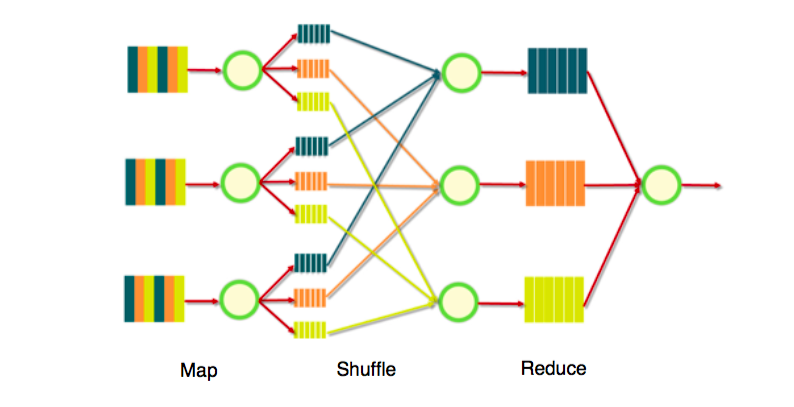
\includegraphics[scale=0.6]{image/MapRed.png}
    \caption{Схема распараллеливание.}
    \label{srg}
\end{figure}

На стадии Map параллельно считываются данные из независимых блоков, на которые
разбит исходный входной файл. Происходит их преобразование в пары (Ключ, Значение).
Затем идет стадия Shuffle: вывод функции Map распределяется по «корзинам», в
зависимости от значения ключа. Все пары (Ключ, Значение), имеющие одинаковый ключ,
попадают в одну корзину и отдаются определенному редьюсеру. Таким образом, данные
из разных частей входного файла могут собраться вместе при обработке на стадии
Reduce. Такая архитектура позволяет быстрое распараллеливание и не загружает
оперативную память, что необходимо при решении поставленной задачи.

Краткая реализация алгоритма DDM в парадигме MapReduce:

\begin{enumerate}
\item Считываются значения вектаров для каждого слова. Для первой эпохи значения
заполняются случайными величинами в диапазоне $[-0.1, 0.1]$.

\item На стадии Map происходит параллельное считывание пар $(u, v, q)$.

\item Формируется пара (Ключ, Значение) для её обработки на стадии Reduce. Ключ = $u$,
Значение = $v$. Отправляются на Reduce.

\item Для каждой такой пары генерируется $q$ негативных примеров гипонимов $u'$ и $q$
негативных примеров гиперонимов $v'$.

\item Для каждой пары $(u, v')$ ( аналогично для $(u', v)$) рассчитывается разница расстояния между $u$ и $v'$ и расстояния между $u$, $v$. Если $f(x) + \log(q) < f(x') + \log(q')$, то необходимо изменить вектора $u, v, v'$ - переход к пункту 4. Иначе просматривается следующая
пара.

\item Рассчитываются антиградиенты $du, dv, dv'$ и умножаются на шаг обучения

\item Формируются пары (Ключ, Значение) для их обработки на стадии Reduce. Ключ
соответствует самому вектору, а значение - изменению. Получаются пары $(u, du)$, $(v,
dv)$, $(v’, dv’)$. Отправляются на Reduce.

\item На стадии Reduce для каждого вектора $u$ (аналогично $v$), собирается список всех
его изменений, полученных из пункта 6 и изначальное значение вектора из пункта 1.

\item Высчитывается новое значение вектора и сохраняется в файле, для его считывания
следующий эпохой.
\end{enumerate}


\subsubsection{Тестирование}

При распараллеливании данного алгоритма на 24 кластера, получилось, что средняя
продолжительность вычисления одной эпохи составляет 50 секунд.
Параметры сети были установлены следующими: длина векора 100, шаг обучения 0.1, кол-
во эпох 100.
Также, как и при исследовании метода Word2Vec были протестированны алгоритмы GBR и
LambdaRank с видами представления векторов: $Diff, Dist1, Dist2, Cos$.
Полученные результаты:

[ТАБЛИЧКА]